\documentclass[10pt,a4paper]{article}
\usepackage[margin=1.8cm]{geometry}
\usepackage[T1]{fontenc}
\usepackage{newtxtext,newtxmath}
\usepackage{tikz,booktabs,xcolor,enumitem,array,tabularx}
\usetikzlibrary{arrows.meta,positioning,shapes.geometric,calc}
\usepackage[hidelinks]{hyperref}
\definecolor{foa}{HTML}{2A78D6}\definecolor{red5}{HTML}{E34948}\definecolor{gnd}{HTML}{333333}
\definecolor{sda}{HTML}{1BAF7A}\definecolor{scl}{HTML}{EDA100}\definecolor{v33}{HTML}{E87BA4}\definecolor{dat}{HTML}{6250D6}
\setlist{itemsep=1pt,topsep=2pt}
\setlength{\parindent}{0pt}\setlength{\parskip}{4pt}
\tikzset{
  blk/.style={draw=black!50,rounded corners=3pt,fill=white,align=center,inner sep=4pt,font=\sffamily\footnotesize},
  stp/.style={draw=foa,rounded corners=3pt,fill=foa!7,align=center,inner sep=4pt,text width=4.2cm,font=\sffamily\footnotesize},
  dec/.style={draw=red5,diamond,aspect=2.4,fill=red5!6,align=center,inner sep=1pt,font=\sffamily\footnotesize},
  arr/.style={-{Stealth[length=4pt]},line width=0.6pt,draw=black!60},
  w/.style={line width=1.1pt},
}
\begin{document}
{\sffamily\color{foa}\small CSD457 · GROUP G-04 · HARDWARE BUILD}\\[2pt]
{\sffamily\bfseries\LARGE FOA testbed: build and run guide}\\[3pt]
{\sffamily Four ESP8266 nodes, one INA226 energy monitor, OLED, DHT22 and LEDs. Rishit Kamboj and Farhan Naik.}

\section*{1. What we are building}
Four ESP8266 boards each run the same FOA firmware: a traffic detector that keeps learning, and that
shares a 92-byte signed update with the other boards over ESP-NOW every learning cycle. The laptop
receives their telemetry, logs everything over USB, and plays the attacker. An INA226 measures how much
energy one node (Node~1) uses per learning cycle.

\begin{center}
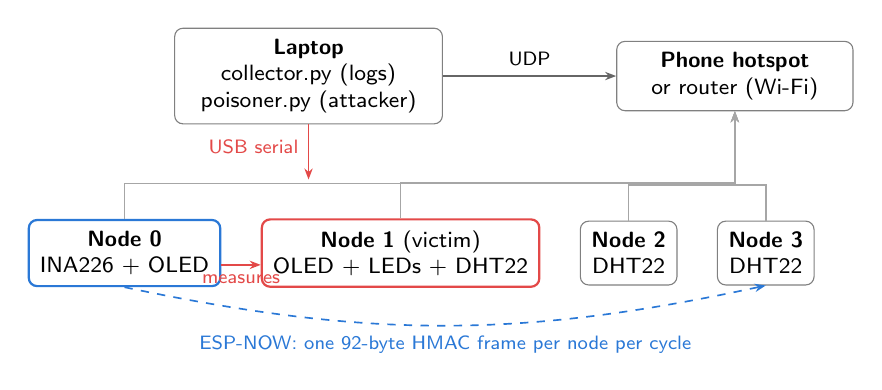
\begin{tikzpicture}[node distance=6mm]
\node[blk,minimum width=3.4cm] (lap) {\textbf{Laptop}\\collector.py (logs)\\poisoner.py (attacker)};
\node[blk,right=2.2cm of lap,minimum width=3cm] (wifi) {\textbf{Phone hotspot}\\or router (Wi-Fi)};
\node[blk,below left=1.2cm and -0.6cm of lap,draw=foa,line width=0.8pt] (n0) {\textbf{Node 0}\\INA226 + OLED};
\node[blk,right=0.5cm of n0,draw=red5,line width=0.8pt] (n1) {\textbf{Node 1} (victim)\\OLED + LEDs + DHT22};
\node[blk,right=0.5cm of n1] (n2) {\textbf{Node 2}\\DHT22};
\node[blk,right=0.5cm of n2] (n3) {\textbf{Node 3}\\DHT22};
\draw[arr,dashed,foa] (n0.south) to[bend right=12] node[below,font=\sffamily\scriptsize,text=foa]{ESP-NOW: one 92-byte HMAC frame per node per cycle} (n3.south);
\foreach \n in {n0,n1,n2,n3} \draw[arr,black!35] (\n.north) -- ($(\n.north)+(0,0.45)$) -| (wifi.south);
\draw[arr] (lap.east) -- node[above,font=\sffamily\scriptsize]{UDP} (wifi.west);
\draw[arr,red5] (lap.south) -- node[left,font=\sffamily\scriptsize,text=red5,pos=0.4]{USB serial} ($(lap.south)+(0,-0.7)$);
\draw[arr,red5,line width=0.9pt] ($(n0.east)+(0,-0.15)$) -- node[below,font=\sffamily\scriptsize,text=red5]{measures} ($(n1.west)+(0,-0.15)$);
\end{tikzpicture}
\end{center}

\section*{2. Parts and roles}
\begin{tabularx}{\linewidth}{@{}lX@{}}
\toprule
Node 0 & ESP8266 + INA226 (energy monitor for Node 1) + OLED (status). Also a normal FOA node.\\
Node 1 & ESP8266, the \textbf{victim}: the board the attacker targets and the INA226 measures. OLED, red and green LEDs, DHT22.\\
Nodes 2, 3 & ESP8266 + DHT22. Peers.\\
Shared & 2 breadboards, jumper wires, 4 USB data cables (one of them modified, Section 4), 220\,$\Omega$ resistors for the LEDs. The 5\,k$\Omega$ resistors are not needed: the INA226 and DHT22 modules have their own pull-ups.\\
Wi-Fi & Phone hotspot or router. Every node and the laptop must be on the same network.\\
\bottomrule
\end{tabularx}

\section*{3. Before wiring}
\begin{enumerate}
\item \textbf{Solder the INA226 header pins} (8 pins, short side through the board, solder on the top).
  Do it in the lab. Unsoldered pins give wrong readings.
\item On the INA226, the big resistor should read \textbf{R100} (0.1\,$\Omega$); the firmware assumes this.
\item Label the boards Node 0 to Node 3 with tape. NodeMCU pin names (D1, D2, ...) are printed on the board.
\end{enumerate}

\section*{4. Wiring}
\textbf{All nodes share one I2C rule:} SDA = \textbf{D2}, SCL = \textbf{D1}, sensors get \textbf{3V3} and \textbf{GND}.
OLED and INA226 sit on the same two I2C wires (they have different addresses, 0x3C and 0x40).

\begin{center}
\small
\begin{tabular}{@{}llll@{}}
\toprule
Part & Part pin & ESP8266 pin & Notes\\
\midrule
INA226 (Node 0) & VCC / GND & 3V3 / GND & \\
 & SDA / SCL & D2 / D1 & \\
 & ALE & not connected & alert pin, unused\\
 & VBS & \textbf{IN$-$} (jumper on the module side) & so it reads Node 1's supply voltage\\
 & IN+ / IN$-$ & see power path below & in series with Node 1's 5\,V\\
OLED SSD1306 (Nodes 0, 1) & VCC / GND & 3V3 / GND & \\
 & SDA / SCL & D2 / D1 & shares the bus with the INA226 on Node 0\\
DHT22 (Nodes 1--3) & + / out / $-$ & 3V3 / \textbf{D5} / GND & module version has its pull-up\\
Red LED (Node 1) & long leg & \textbf{D6} through 220\,$\Omega$ & short leg to GND\\
Green LED (Node 1) & long leg & \textbf{D7} through 220\,$\Omega$ & short leg to GND\\
\bottomrule
\end{tabular}
\end{center}

\textbf{Power path for the measurement (Node 1).} Take Node 1's own USB data cable. Carefully open it
in the middle and \textbf{cut only the red wire} (5\,V). Leave the data wires (white, green) and the black
ground wire intact, so Node 1 still talks to the laptop. Connect the red wire from the \textbf{laptop side}
to \textbf{IN+} and the red wire from the \textbf{board side} to \textbf{IN$-$}. All the current Node 1
draws now flows through the 0.1\,$\Omega$ shunt.

\begin{center}
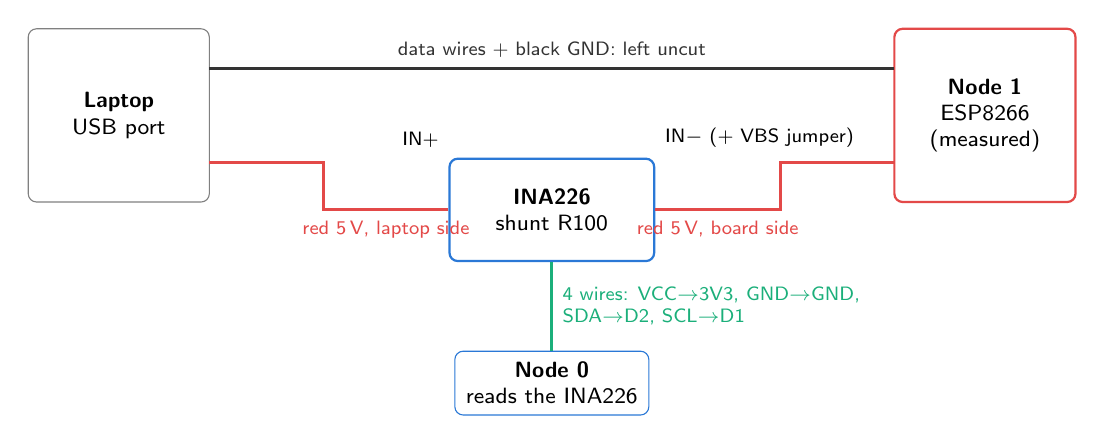
\begin{tikzpicture}[x=1cm,y=1cm]
\node[blk,minimum width=2.3cm,minimum height=2.2cm] (lap) at (0,0) {\textbf{Laptop}\\USB port};
\node[blk,draw=foa,line width=0.8pt,minimum width=2.6cm,minimum height=1.3cm] (ina) at (5.5,-1.2) {\textbf{INA226}\\shunt R100};
\node[blk,draw=red5,line width=0.8pt,minimum width=2.3cm,minimum height=2.2cm] (n1) at (11,0) {\textbf{Node 1}\\ESP8266\\(measured)};
\draw[w,gnd] (1.15,0.6) -- node[above,font=\sffamily\scriptsize]{data wires + black GND: left uncut} (9.85,0.6);
\draw[w,red5] (1.15,-0.6) -- (2.6,-0.6) |- node[pos=0.75,below,font=\sffamily\scriptsize,text=red5]{red 5\,V, laptop side} (ina.west);
\draw[w,red5] (ina.east) -| node[pos=0.25,below,font=\sffamily\scriptsize,text=red5]{red 5\,V, board side} (8.4,-0.6) -- (9.85,-0.6);
\node[font=\sffamily\scriptsize,anchor=south east] at (ina.north west) {IN+};
\node[font=\sffamily\scriptsize,anchor=south west] at (ina.north east) {IN$-$ (+ VBS jumper)};
\node[blk,draw=foa,minimum width=2.3cm] (n0) at (5.5,-3.4) {\textbf{Node 0}\\reads the INA226};
\draw[w,sda] (ina.south) -- node[right,font=\sffamily\scriptsize,align=left]{4 wires: VCC$\to$3V3, GND$\to$GND,\\SDA$\to$D2, SCL$\to$D1} (n0.north);
\end{tikzpicture}
\end{center}


\newpage
\section*{4b. Full circuit diagram}
\begin{center}
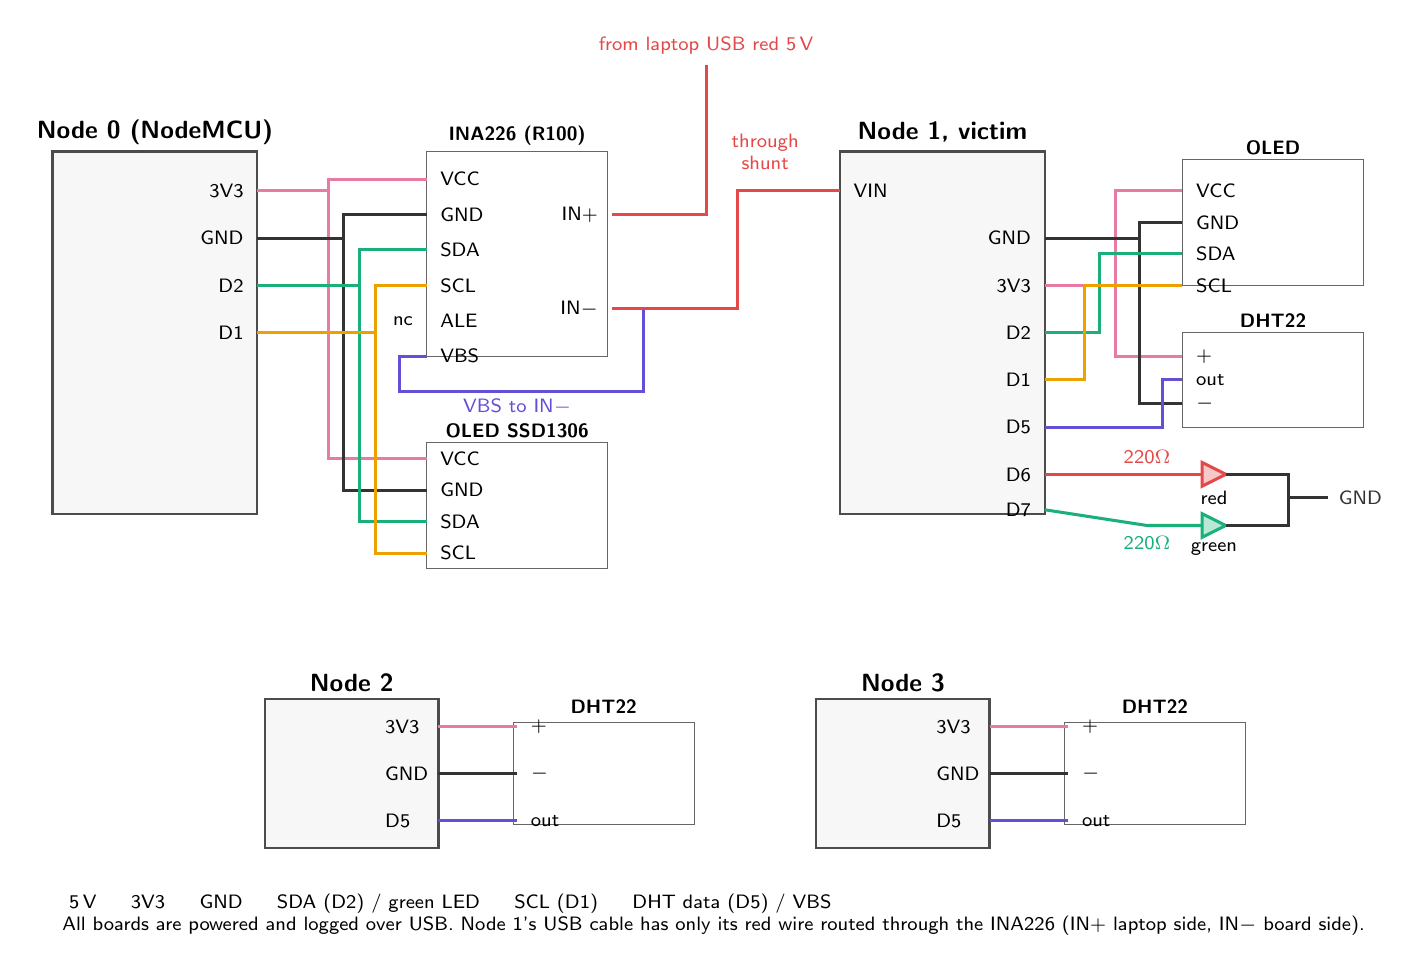
\begin{tikzpicture}[x=1cm,y=1cm,
  mcu/.style={draw=black!70,line width=0.8pt,fill=black!3,minimum width=2.6cm,minimum height=4.6cm},
  mod/.style={draw=black!60,fill=white,minimum width=2.3cm,align=center,font=\sffamily\scriptsize},
  pl/.style={font=\sffamily\scriptsize},
  dot/.style={circle,fill,inner sep=1pt}]
% ---------- Node 0
\node[mcu] (A) at (0,0) {};
\node[font=\sffamily\bfseries\small] at (0,2.55) {Node 0 (NodeMCU)};
\foreach \y/\p in {1.8/3V3,1.2/GND,0.6/D2,0.0/D1} {\node[pl,anchor=east] at (1.25,\y) {\p}; \coordinate (A\p) at (1.3,\y);}
\node[mod,minimum height=2.6cm] (INA) at (4.6,1.0) {};
\node[font=\sffamily\bfseries\scriptsize] at (4.6,2.5) {INA226 (R100)};
\foreach \y/\p in {1.95/VCC,1.5/GND,1.05/SDA,0.6/SCL,0.15/ALE,-0.3/VBS} {\node[pl,anchor=west] at (3.5,\y) {\p}; \coordinate (I\p) at (3.45,\y);}
\node[pl,anchor=east] at (5.75,1.5) {IN+}; \coordinate (IINp) at (5.8,1.5);
\node[pl,anchor=east] at (5.75,0.3) {IN$-$}; \coordinate (IINm) at (5.8,0.3);
\node[mod,minimum height=1.6cm] (OL0) at (4.6,-2.2) {};
\node[font=\sffamily\bfseries\scriptsize] at (4.6,-1.25) {OLED SSD1306};
\foreach \y/\p in {-1.6/VCC,-2.0/GND,-2.4/SDA,-2.8/SCL} {\node[pl,anchor=west] at (3.5,\y) {\p}; \coordinate (O\p) at (3.45,\y);}
\draw[w,v33] (A3V3) -- (2.2,1.8) |- (IVCC); \draw[w,v33] (2.2,1.8) |- (OVCC);
\draw[w,gnd] (AGND) -- (2.4,1.2) |- (IGND); \draw[w,gnd] (2.4,1.2) |- (OGND);
\draw[w,sda] (AD2) -- (2.6,0.6) |- (ISDA); \draw[w,sda] (2.6,0.6) |- (OSDA);
\draw[w,scl] (AD1) -- (2.8,0.0) |- (ISCL); \draw[w,scl] (2.8,0.0) |- (OSCL);
\node[pl,anchor=east] at (3.4,0.15) {nc};
\draw[w,dat] (IVBS) -- (3.1,-0.3) -- (3.1,-0.75) -- (6.2,-0.75) -- (6.2,0.3) -- (IINm);
\node[pl,text=dat] at (4.6,-0.95) {VBS to IN$-$};
% ---------- Node 1
\node[mcu] (B) at (10,0) {};
\node[font=\sffamily\bfseries\small] at (10,2.55) {Node 1, victim};
\node[pl,anchor=west] at (8.75,1.8) {VIN}; \coordinate (BVIN) at (8.7,1.8);
\foreach \y/\p in {1.2/GND,0.6/3V3,0.0/D2,-0.6/D1,-1.2/D5,-1.8/D6,-2.25/D7} {\node[pl,anchor=east] at (11.25,\y) {\p}; \coordinate (B\p) at (11.3,\y);}
\draw[w,red5] (IINp) -- (7.0,1.5) -- (7.0,3.4) node[above,pl,text=red5]{from laptop USB red 5\,V};
\draw[w,red5] (IINm) -- (7.4,0.3) -- (7.4,1.8) -- (BVIN);
\node[pl,text=red5,align=center] at (7.75,2.3) {through\\shunt};
% Node 1 peripherals (right side)
\node[mod,minimum height=1.6cm] (OL1) at (14.2,1.4) {}; \node[font=\sffamily\bfseries\scriptsize] at (14.2,2.35) {OLED};
\node[mod,minimum height=1.2cm] (DH1) at (14.2,-0.6) {}; \node[font=\sffamily\bfseries\scriptsize] at (14.2,0.15) {DHT22};
\coordinate (Br) at (11.3,0);
\foreach \y/\c/\lab in {1.8/v33/VCC,1.4/gnd/GND,1.0/sda/SDA,0.6/scl/SCL} \node[pl,anchor=west] at (13.1,\y) {\lab};
\foreach \y/\lab in {-0.3/+,-0.6/out,-0.9/$-$} \node[pl,anchor=west] at (13.1,\y) {\lab};
\draw[w,v33] (B3V3) -- (12.2,0.6) |- (13.05,1.8); \draw[w,v33] (12.2,0.6) |- (13.05,-0.3);
\draw[w,gnd] (BGND) -- (12.5,1.2) |- (13.05,1.4); \draw[w,gnd] (12.5,1.2) |- (13.05,-0.9);
\draw[w,sda] (BD2) -- (12.0,0.0) |- (13.05,1.0);
\draw[w,scl] (BD1) -- (11.8,-0.6) |- (13.05,0.6);
\draw[w,dat] (BD5) -- (12.8,-1.2) |- (13.05,-0.6);
% LEDs
\draw[w,red5] (BD6) -- (12.6,-1.8) node[pl,above]{220$\Omega$} -- (13.3,-1.8);
\draw[w,red5,fill=red5!30] (13.3,-1.65) -- (13.6,-1.8) -- (13.3,-1.95) -- cycle; \node[pl] at (13.45,-2.1) {red};
\draw[w,sda] (BD7) -- (12.6,-2.45) node[pl,below]{220$\Omega$} -- (13.3,-2.45);
\draw[w,sda,fill=sda!30] (13.3,-2.3) -- (13.6,-2.45) -- (13.3,-2.6) -- cycle; \node[pl] at (13.45,-2.75) {green};
\draw[w,gnd] (13.6,-1.8) -- (14.4,-1.8) -- (14.4,-2.45) -- (13.6,-2.45); \draw[w,gnd] (14.4,-2.1) -- (14.9,-2.1) node[right,pl]{GND};
% ---------- Nodes 2 and 3
\foreach \x/\n in {2.5/2,9.5/3} {
  \node[draw=black!70,line width=0.8pt,fill=black!3,minimum width=2.2cm,minimum height=1.9cm] at (\x,-5.6) {};
  \node[font=\sffamily\bfseries\small] at (\x,-4.45) {Node \n};
  \foreach \y/\p in {-5.0/3V3,-5.6/GND,-6.2/D5} \node[pl,anchor=west] at (\x+0.3,\y) {\p};
  \node[mod,minimum height=1.3cm] at (\x+3.2,-5.6) {}; \node[font=\sffamily\bfseries\scriptsize] at (\x+3.2,-4.75) {DHT22};
  \foreach \y/\l in {-5.0/+,-5.6/$-$,-6.2/out} \node[pl,anchor=west] at (\x+2.15,\y) {\l};
  \draw[w,v33] (\x+1.1,-5.0) -- (\x+2.1,-5.0); \draw[w,gnd] (\x+1.1,-5.6) -- (\x+2.1,-5.6); \draw[w,dat] (\x+1.1,-6.2) -- (\x+2.1,-6.2);
}
\node[pl,align=left,anchor=north west] at (-1.3,-7.0) {\textcolor{red5}{$\blacksquare$} 5\,V \quad \textcolor{v33}{$\blacksquare$} 3V3 \quad \textcolor{gnd}{$\blacksquare$} GND \quad \textcolor{sda}{$\blacksquare$} SDA (D2) / green LED \quad \textcolor{scl}{$\blacksquare$} SCL (D1) \quad \textcolor{dat}{$\blacksquare$} DHT data (D5) / VBS\\
All boards are powered and logged over USB. Node 1's USB cable has only its red wire routed through the INA226 (IN+ laptop side, IN$-$ board side).};
\end{tikzpicture}
\end{center}

\newpage
\section*{5. Software and flashing}
\begin{enumerate}
\item Laptop and boards on the same Wi-Fi. Find the laptop's IP (System Settings $\to$ Wi-Fi $\to$ Details).
\item In \texttt{firmware/esp8266\_foa/foa\_config.h} set \texttt{WIFI\_SSID}, \texttt{WIFI\_PASS} and
  \texttt{COLLECTOR\_IP} (laptop IP, written with commas, e.g.\ \texttt{192, 168, 43, 20}). Do not commit the password.
\item Plug in one board, find its port: \texttt{ls /dev/cu.usb*}
\item Flash it (repeat for \texttt{NODE\_ID=1, 2, 3}, one board at a time):
\end{enumerate}
{\small\begin{verbatim}
bash firmware/flash_esp8266.sh /dev/cu.usbserial-XXXX 0
\end{verbatim}}
\begin{enumerate}[resume]
\item Check it: \texttt{arduino-cli monitor -p /dev/cu.usbserial-XXXX -c baudrate=115200}. The first line
  should read \texttt{BOOT,0,wifi=1,...,ina226=1,oled=1}. Node 0 then prints \texttt{PWR} lines.
\end{enumerate}

\section*{6. What the firmware does}
\begin{center}
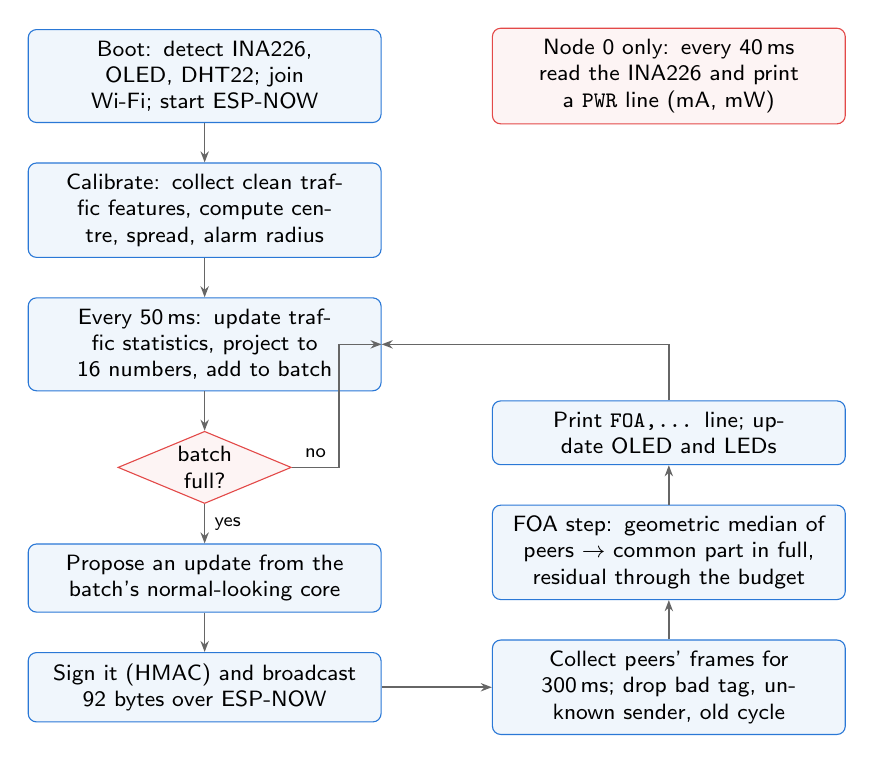
\begin{tikzpicture}[node distance=5mm]
\node[stp] (boot) {Boot: detect INA226, OLED, DHT22; join Wi-Fi; start ESP-NOW};
\node[stp,below=of boot] (cal) {Calibrate: collect clean traffic features, compute centre, spread, alarm radius};
\node[stp,below=of cal] (samp) {Every 50\,ms: update traffic statistics, project to 16 numbers, add to batch};
\node[dec,below=of samp] (full) {batch\\full?};
\node[stp,below=of full] (prop) {Propose an update from the batch's normal-looking core};
\node[stp,below=of prop] (send) {Sign it (HMAC) and broadcast 92 bytes over ESP-NOW};
\node[stp,right=1.4cm of send] (recv) {Collect peers' frames for 300\,ms; drop bad tag, unknown sender, old cycle};
\node[stp,above=of recv] (foa) {FOA step: geometric median of peers $\to$ common part in full, residual through the budget};
\node[stp,above=of foa] (log) {Print \texttt{FOA,...} line; update OLED and LEDs};
\draw[arr] (boot) -- (cal); \draw[arr] (cal) -- (samp); \draw[arr] (samp) -- (full);
\draw[arr] (full) -- node[right,font=\sffamily\scriptsize]{yes} (prop);
\draw[arr] (full.east) -- node[above,font=\sffamily\scriptsize]{no} ++(0.6,0) |- (samp.east);
\draw[arr] (prop) -- (send); \draw[arr] (send) -- (recv); \draw[arr] (recv) -- (foa); \draw[arr] (foa) -- (log);
\draw[arr] (log.north) |- (samp.east);
\node[stp,right=1.4cm of boot,draw=red5,fill=red5!6] (pwr) {Node 0 only: every 40\,ms read the INA226 and print a \texttt{PWR} line (mA, mW)};
\end{tikzpicture}
\end{center}

\section*{7. Experiment day}
\begin{center}
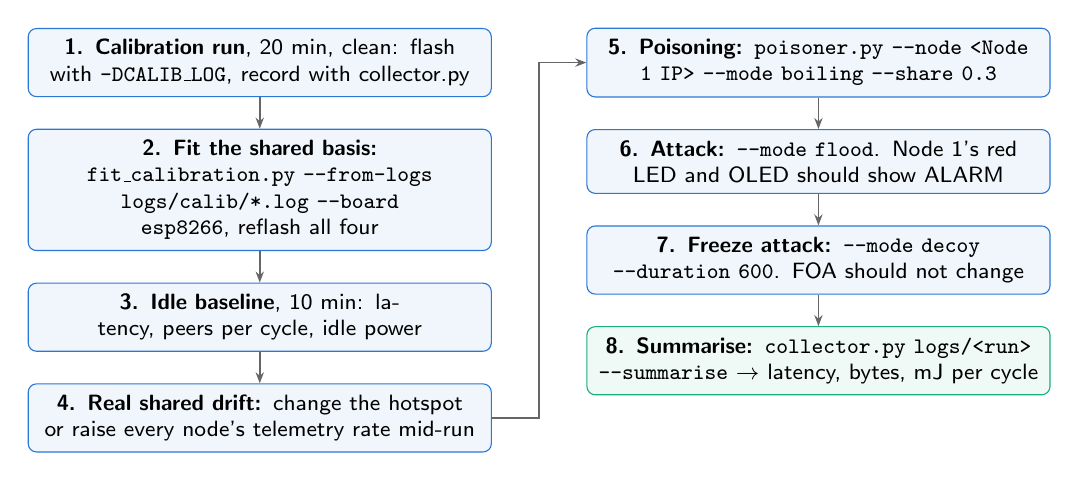
\begin{tikzpicture}[node distance=4mm]
\node[stp,text width=5.6cm] (a) {\textbf{1. Calibration run}, 20 min, clean: flash with \texttt{-DCALIB\_LOG}, record with collector.py};
\node[stp,text width=5.6cm,below=of a] (b) {\textbf{2. Fit the shared basis:} \texttt{fit\_calibration.py --from-logs logs/calib/*.log --board esp8266}, reflash all four};
\node[stp,text width=5.6cm,below=of b] (c) {\textbf{3. Idle baseline}, 10 min: latency, peers per cycle, idle power};
\node[stp,text width=5.6cm,below=of c] (d) {\textbf{4. Real shared drift:} change the hotspot or raise every node's telemetry rate mid-run};
\node[stp,text width=5.6cm,right=1.2cm of a] (e) {\textbf{5. Poisoning:} \texttt{poisoner.py --node <Node 1 IP> --mode boiling --share 0.3}};
\node[stp,text width=5.6cm,below=of e] (f) {\textbf{6. Attack:} \texttt{--mode flood}. Node 1's red LED and OLED should show ALARM};
\node[stp,text width=5.6cm,below=of f] (g) {\textbf{7. Freeze attack:} \texttt{--mode decoy --duration 600}. FOA should not change};
\node[stp,text width=5.6cm,below=of g,draw=sda,fill=sda!7] (h) {\textbf{8. Summarise:} \texttt{collector.py logs/<run> --summarise} $\to$ latency, bytes, mJ per cycle};
\draw[arr] (a) -- (b); \draw[arr] (b) -- (c); \draw[arr] (c) -- (d); \draw[arr] (d.east) -- ++(0.6,0) |- (e.west);
\draw[arr] (e) -- (f); \draw[arr] (f) -- (g); \draw[arr] (g) -- (h);
\end{tikzpicture}
\end{center}
Run the collector in a second terminal during every step:
{\small\begin{verbatim}
pip3 install pyserial
python3 firmware/laptop/collector.py logs/run1 --serial /dev/cu.usbserial-A /dev/cu.usbserial-B ...
\end{verbatim}}

\section*{8. If something does not work}
\begin{tabularx}{\linewidth}{@{}lX@{}}
\toprule
\texttt{wifi=0} & Wrong SSID or password; the ESP8266 only joins 2.4\,GHz networks (turn on 2.4\,GHz / "maximise compatibility" on the hotspot).\\
\texttt{ina226=0} & Check SDA $\to$ D2, SCL $\to$ D1, 3V3 and GND; resolder the header.\\
\texttt{peers 0} & Boards on different Wi-Fi networks or channels; all must join the same hotspot.\\
\texttt{PWR} current near 0 & Node 1 still gets 5\,V around the shunt: only the red wire must go through IN+/IN$-$.\\
OLED blank & Address must be 0x3C; check the wires are on D1/D2.\\
Board resets & Weak cable or hub; use the laptop port directly.\\
\bottomrule
\end{tabularx}
\end{document}
